\chapter{Tools demonstration}
\label{cap:casestudy}

To illustrate the whole process of generating test cases and extracting formal properties and how our implemented tools work, we will use as an example the statechart model given in \ref{webOrderProc} created with the Yakindu Statechart Tools \cite{Yakindu}. It models the order processing of an ecommerce portal after the user concluded the purchase. An order is made of entries, each one containing a product and its corresponding quantity. The order information must be converted in a XML file that will be sent to an integration layer. In parallel to the XML preparation, a job is executed to send customers an email informing that their order was received and is being processed.

\begin{figure}[htb]
\centering
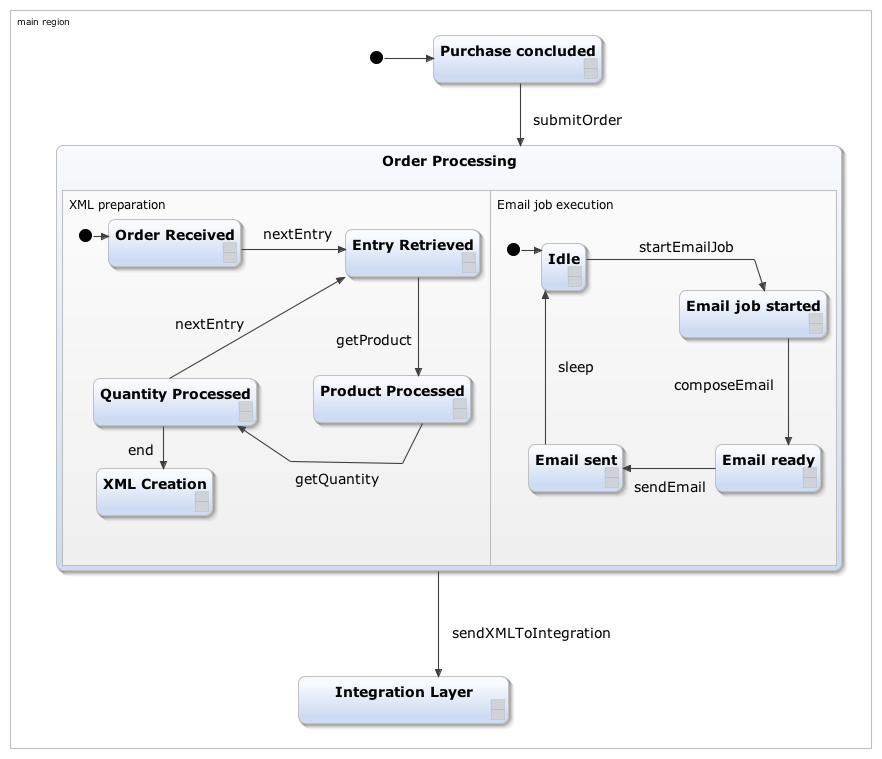
\includegraphics[width=15cm]{figuras/webOrderProc}
\caption{\label{webOrderProc}Statechart model for order processing}
\end{figure}

\section{Test case generation tool}

The interface of test generation tool is displayed in figure \ref{testGenClean}.

\begin{figure}[htb]
\centering
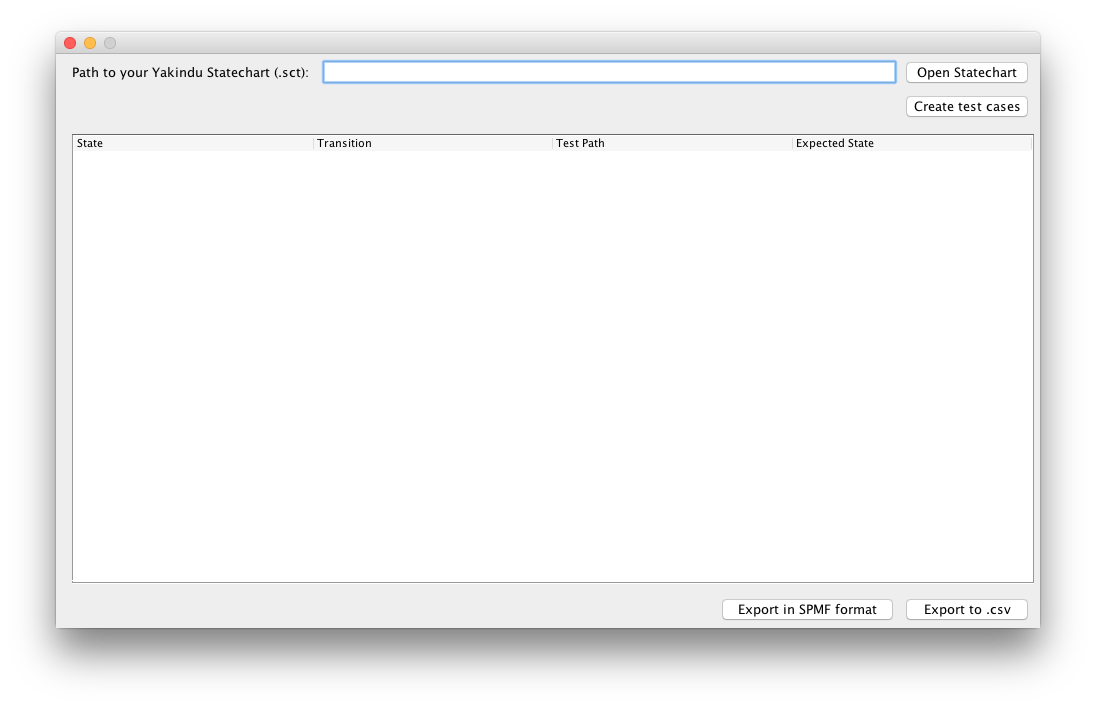
\includegraphics[width=\textwidth]{figuras/testGenClean}
\caption{\label{testGenClean} Test case generator interface.}
\end{figure}

We start by opening the statechart we created. Then, we click on button \textit{Create test cases} and the created test cases will be outputted in the screen, as shown in figure \ref{testGenResults}. Note that the table is divided in four columns: 
\begin{itemize}
\item \textit{State}, which tells from which state we are taking a transition
\item \textit{Transition}, which informs the transition that is being tested 
\item \textit{Test path}, which contains the path to execute that transition
\item \textit{Expected state}, which is the expected state we should get when that transition is taken
\end{itemize}

\begin{figure}[htb]
\centering
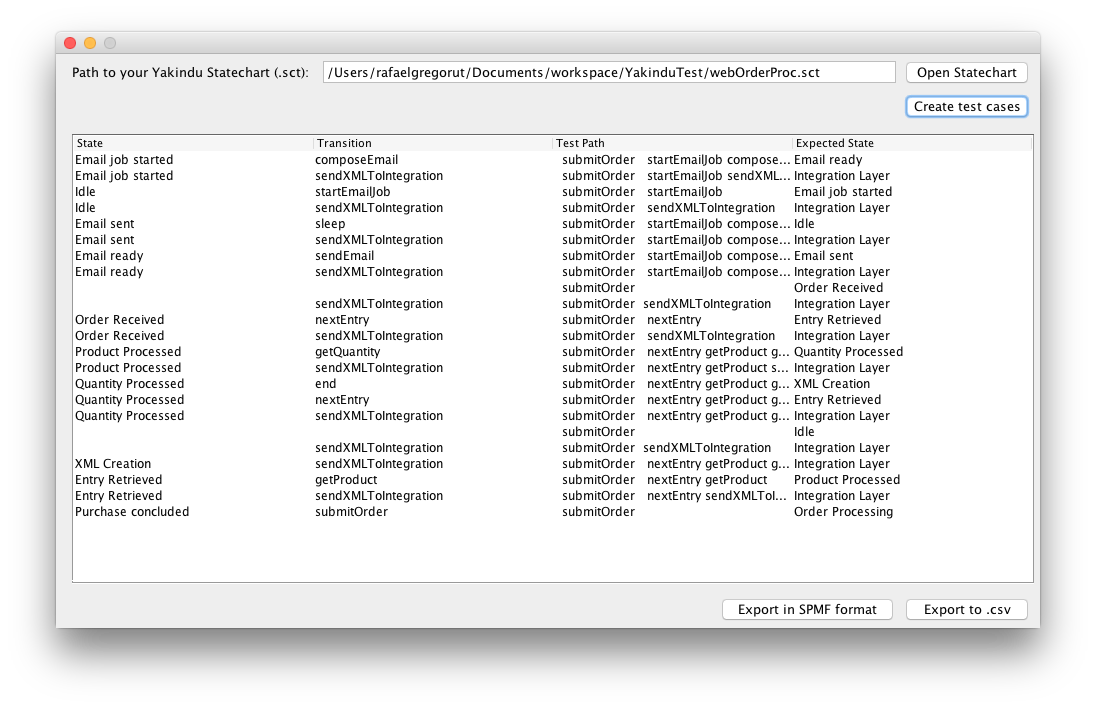
\includegraphics[width=\textwidth]{figuras/testGenResults}
\caption{\label{testGenResults} Test cases created for statechart \ref{webOrderProc}.}
\end{figure}

If we click to \textit{export in SPMF format}, we are able to save the test paths in a text file with the format that the framework $SPMF$ and our second tool need as input. Test paths are then saved in the way displayed by figure \ref{resultsSPMFFile}.

\begin{figure}[htb]
\centering
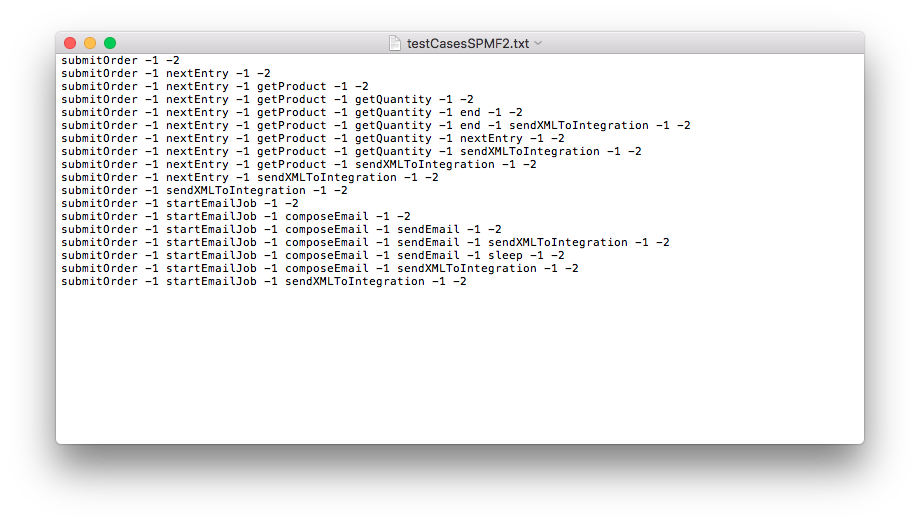
\includegraphics[width=\textwidth]{figuras/resultsSPMFFile}
\caption{\label{resultsSPMFFile} Test paths from \ref{webOrderProc} in the SPMF input format.}
\end{figure}

We are also capable to export the information from all columns to a \textit{.csv} file, which can be read by most spreadsheet softwares in the market. Just click on button \textit{Export to .csv}.

The Java code written to develop this tool can be found in our Github repository\footnote{\url{https://github.com/rafaelgregorut/StatechartTests}}.

\section{Formal property specification tool}

The interface of our formal property specification tool is displayed in figure \ref{propGenClean}. It contains two tabs: 
\begin{itemize}
\item \textit{Properties based on test case mining}, where properties will be specified based on the results returned by sequential mining
\item \textit{Properties for specific events}, where the user is able to specify an event and properties related to it will be displayed.
\end{itemize}

\begin{figure}[htb]
\centering
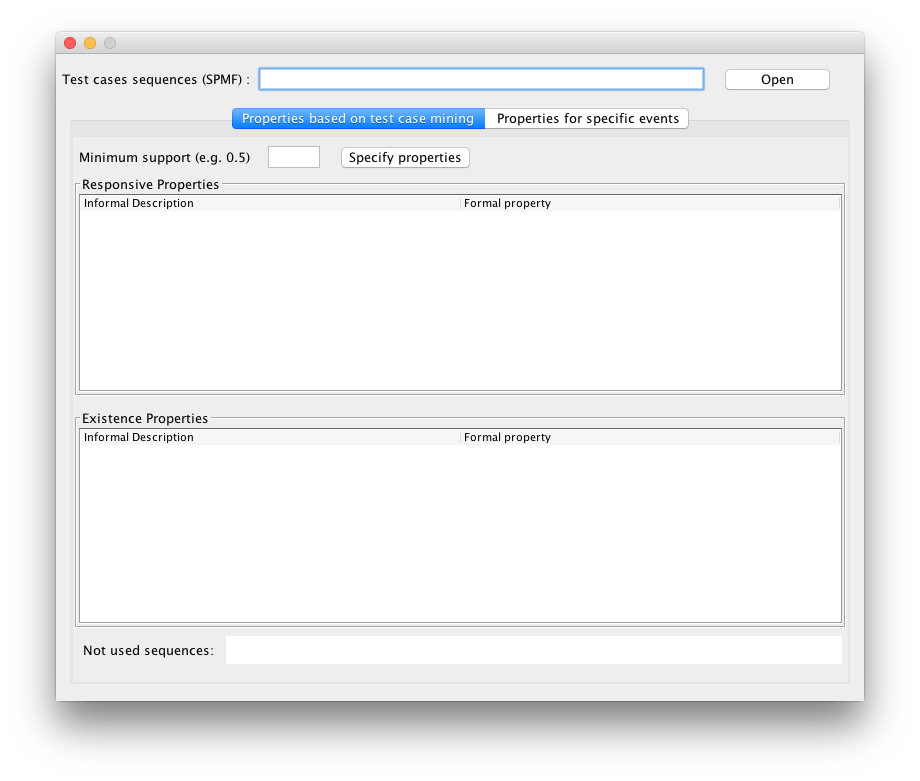
\includegraphics[width=\textwidth]{figuras/propGenClean}
\caption{\label{propGenClean} Property generator tool interface.}
\end{figure}

Initially, we open the file created by our test case generator in $SPMF$ input format, pass a minimum support of 0.3 ($30\%$) and click on \textit{Specify properties} to generate the properties, as displayed in figure \ref{propGenMining}

\begin{figure}[htb]
\centering
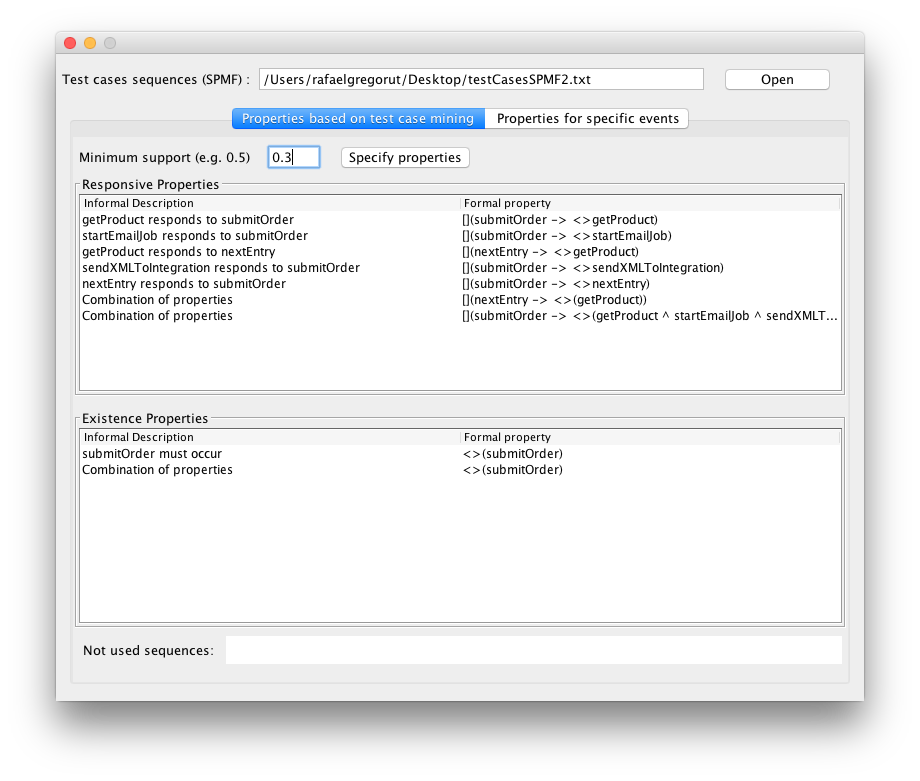
\includegraphics[width=\textwidth]{figuras/propGenMining}
\caption{\label{propGenMining} Properties automatically specified for \ref{webOrderProc} based on the mining of \ref{resultsSPMFFile}.}
\end{figure}

Response properties are displayed in the first panel, note that combined properties are also displayed. Existence properties are shown in the second panel, notice that their combination are displayed too. In both panels there are two columns: 
\begin{itemize}
\item \textit{Informal description}, that contains a description of the property in natural language
\item \textit{Formal property}, where the formal specification in LTL is displayed.
\end{itemize}

Notice that, in case a sequence is ignored in the mining process, its ID will be displayed in the bottom area \textit{Not used sequences}. The ID of a sequence corresponds to the line number where the sequence is located.

If we change to tab \textit{Properties for specific events}, we can obtain response properties for a specific event. In our example, we passed as input the event \textit{sendEmail} and, once \textit{Specify properties} is clicked, the response properties are displayed as shown in figure \ref{propGenSpec}. Note that combined properties are also displayed.


\begin{figure}[htb]
\centering
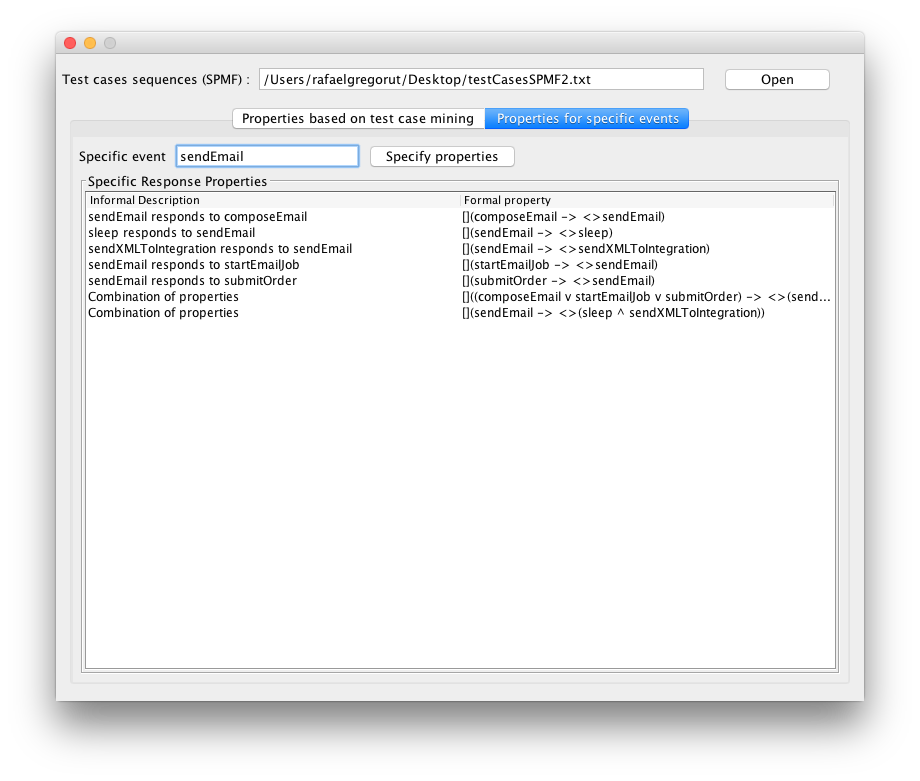
\includegraphics[width=\textwidth]{figuras/propGenSpec}
\caption{\label{propGenSpec} Properties specified for \textit{sendEmail} event.}
\end{figure}

The Java code written to develop this tool can be found in our Github repository\footnote{\url{https://github.com/rafaelgregorut/ExtractingStateSequences}}.

